% Q, K, V diagram: how "its" attends to the earlier words in "The dog wagged its"
% Compile with:
%   pdflatex qkv.tex
%   convert -density 200 qkv.pdf -quality 95 qkv.png

\documentclass[tikz,border=10pt]{standalone}
\usepackage{tikz}
\usetikzlibrary{arrows.meta,positioning,calc}

\definecolor{querycol}{RGB}{190,50,50}    % red   - query
\definecolor{keycol}  {RGB}{50,100,180}   % blue  - keys
\definecolor{valcol}  {RGB}{50,140,80}    % green - values

\begin{document}
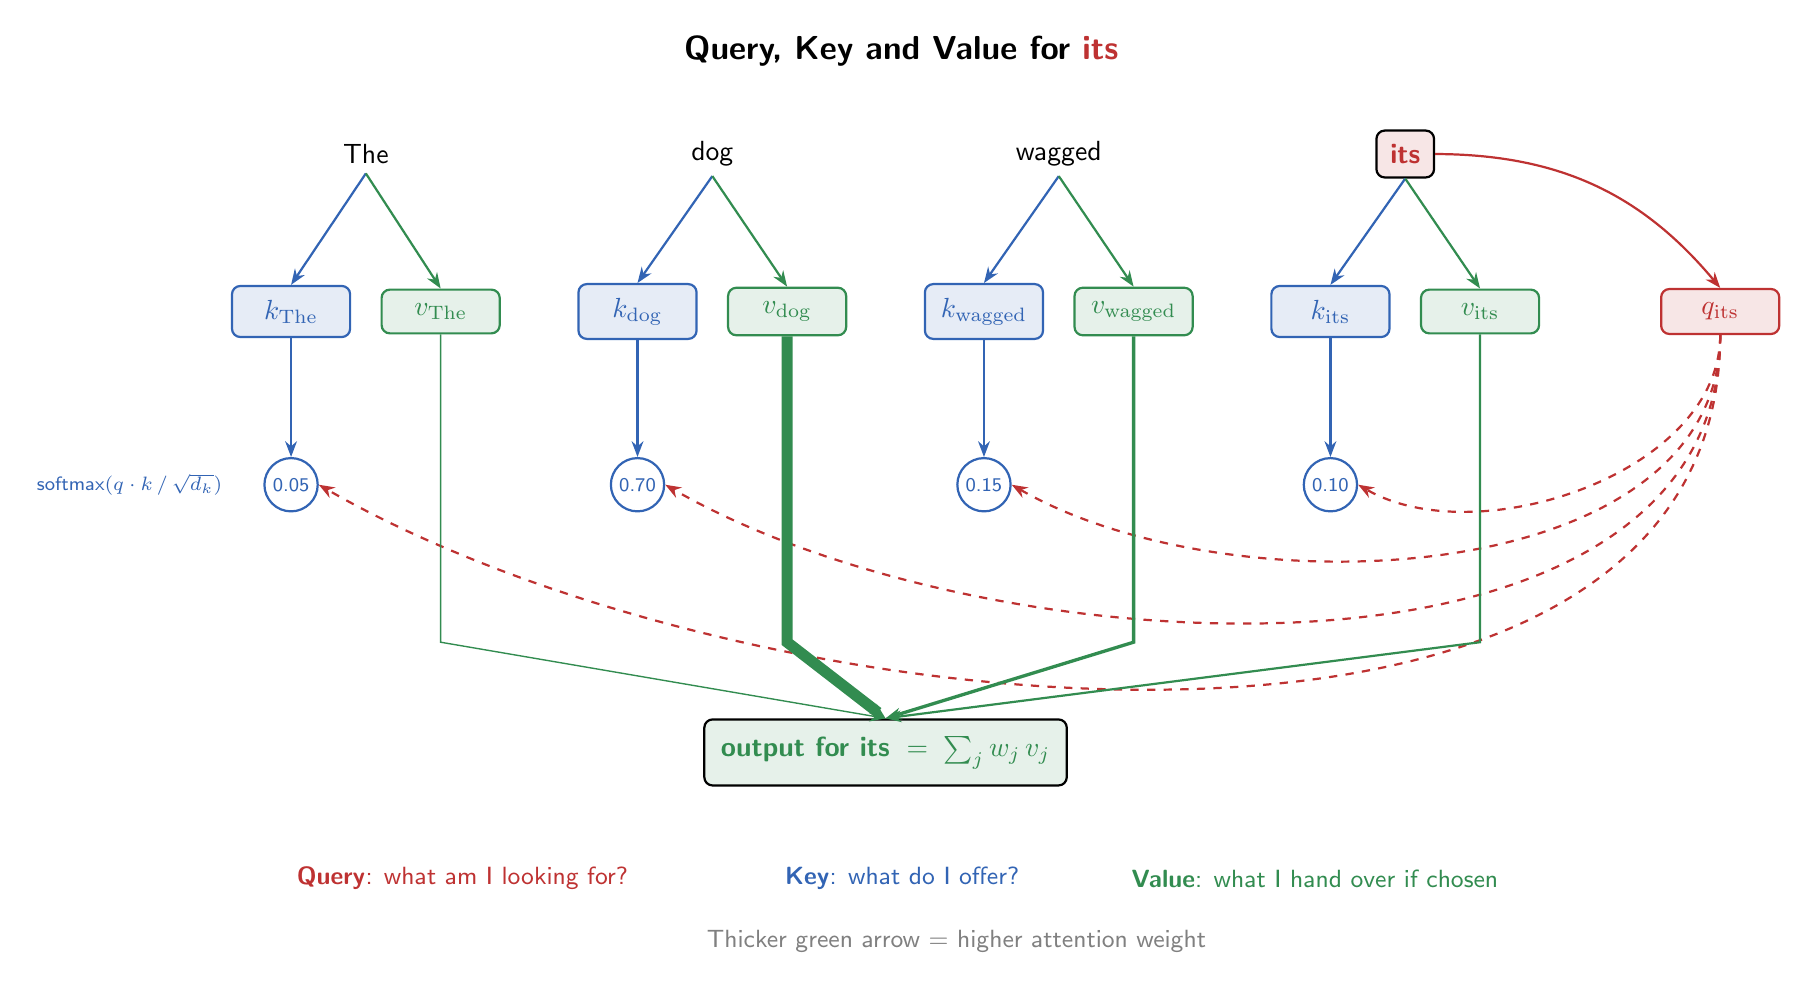
\begin{tikzpicture}[font=\sffamily,
  proj/.style={draw, rounded corners=3pt, thick, inner sep=5pt, minimum width=1.5cm},
  qbox/.style={proj, draw=querycol, fill=querycol!12, text=querycol},
  kbox/.style={proj, draw=keycol,   fill=keycol!12,   text=keycol},
  vbox/.style={proj, draw=valcol,   fill=valcol!12,   text=valcol},
  score/.style={circle, draw=keycol, fill=white, thick, inner sep=2pt, font=\scriptsize\sffamily, text=keycol}]

% -- Title -------------------------------------------------------
\node[font=\large\bfseries\sffamily] at (6.8, 1.3)
    {Query, Key and Value for \textcolor{querycol}{\textbf{its}}};

% -- Words -------------------------------------------------------
\node (w0) at (0,   0) {The};
\node (w1) at (4.4, 0) {dog};
\node (w2) at (8.8, 0) {wagged};
\node[draw, rounded corners=3pt, fill=querycol!12, text=querycol,
      inner sep=5pt, thick] (w3) at (13.2, 0) {\textbf{its}};

% -- Keys and values for every word ------------------------------
\foreach \i/\w in {0/The, 1/dog, 2/wagged, 3/its} {
  \pgfmathsetmacro{\x}{4.4*\i}
  \node[kbox] (k\i) at ({\x-0.95}, -2) {$k_{\mathrm{\w}}$};
  \node[vbox] (v\i) at ({\x+0.95}, -2) {$v_{\mathrm{\w}}$};
  \draw[-{Stealth[length=2mm]}, keycol, thick] (w\i.south) -- (k\i.north);
  \draw[-{Stealth[length=2mm]}, valcol, thick] (w\i.south) -- (v\i.north);
}

% -- Query: only for the word being predicted --------------------
\node[qbox] (q) at (17.2, -2) {$q_{\mathrm{its}}$};
\draw[-{Stealth[length=2mm]}, querycol, thick]
    (w3.east) to[bend left=25] (q.north);

% -- Scores: q . k for each key -----------------------------------
\foreach \i/\s in {0/0.05, 1/0.70, 2/0.15, 3/0.10} {
  \node[score] (s\i) at ({4.4*\i-0.95}, -4.2) {\s};
  \draw[-{Stealth[length=2mm]}, keycol, thick] (k\i.south) -- (s\i.north);
  \draw[-{Stealth[length=2mm]}, querycol, dashed, thick]
      (q.south) to[out=-90, in=-30, looseness=0.9] (s\i.east);
}
\node[font=\scriptsize\sffamily, text=keycol, anchor=east] at (-1.7, -4.2)
    {softmax$(q\cdot k\,/\,\sqrt{d_k})$};

% -- Output: weighted sum of values --------------------------------
\node[draw, rounded corners=3pt, thick, fill=valcol!12, text=valcol,
      inner sep=6pt] (out) at (6.6, -7.6)
    {\textbf{output for \textit{its}} $\;=\; \sum_j w_j\, v_j$};

\foreach \i/\w/\lw in {0/0.05/0.5pt, 1/0.70/4pt, 2/0.15/1.2pt, 3/0.10/0.8pt} {
  \draw[-{Stealth[length=2mm]}, valcol, line width=\lw]
      (v\i.south) -- ($(v\i.south |- 0,-6.2)$) -- (out.north);
}

% -- Legend ------------------------------------------------------
\node[font=\small\sffamily, text=querycol, anchor=west] at (-1.0, -9.2)
    {\textbf{Query}: what am I looking for?};
\node[font=\small\sffamily, text=keycol, anchor=west] at (5.2, -9.2)
    {\textbf{Key}: what do I offer?};
\node[font=\small\sffamily, text=valcol, anchor=west] at (9.6, -9.2)
    {\textbf{Value}: what I hand over if chosen};
\node[font=\small\sffamily, text=gray] at (7.5, -10.0)
    {Thicker green arrow = higher attention weight};

\end{tikzpicture}
\end{document}
